\documentclass[noauthor,nooutcomes,12pt,handout]{ximera}

\graphicspath{  
{./}
{./whoAreYou/}
{./drawingWithTheTurtle/}
{./bisectionMethod/}
{./circles/}
{./anglesAndRightTriangles/}
{./lawOfSines/}
{./lawOfCosines/}
{./plotter/}
{./staircases/}
{./pitch/}
{./qualityControl/}
{./symmetry/}
{./nGonBlock/}
}


%% page layout
\usepackage[cm,headings]{fullpage}
\raggedright
\setlength\headheight{13.6pt}


%% fonts
\usepackage{euler}

\usepackage{FiraMono}
\renewcommand\familydefault{\ttdefault} 
\usepackage[defaultmathsizes]{mathastext}
\usepackage[htt]{hyphenat}

\usepackage[T1]{fontenc}
\usepackage[scaled=1]{FiraSans}

%\usepackage{wedn}
\usepackage{pbsi} %% Answer font


\usepackage{cancel} %% strike through in pitch/pitch.tex


%% \usepackage{ulem} %% 
%% \renewcommand{\ULthickness}{2pt}% changes underline thickness

\tikzset{>=stealth}

\usepackage{adjustbox}

\setcounter{titlenumber}{-1}

%% journal style
\makeatletter
\newcommand\journalstyle{%
  \def\activitystyle{activity-chapter}
  \def\maketitle{%
    \addtocounter{titlenumber}{1}%
                {\flushleft\small\sffamily\bfseries\@pretitle\par\vspace{-1.5em}}%
                {\flushleft\LARGE\sffamily\bfseries\thetitlenumber\hspace{1em}\@title \par }%
                {\vskip .6em\noindent\textit\theabstract\setcounter{question}{0}\setcounter{sectiontitlenumber}{0}}%
                    \par\vspace{2em}
                    \phantomsection\addcontentsline{toc}{section}{\thetitlenumber\hspace{1em}\textbf{\@title}}%
                     }}
\makeatother



%% thm like environments
\let\question\relax
\let\endquestion\relax

\newtheoremstyle{QuestionStyle}{\topsep}{\topsep}%%% space between body and thm
		{}                      %%% Thm body font
		{}                              %%% Indent amount (empty = no indent)
		{\bfseries}            %%% Thm head font
		{)}                              %%% Punctuation after thm head
		{ }                           %%% Space after thm head
		{\thmnumber{#2}\thmnote{ \bfseries(#3)}}%%% Thm head spec
\theoremstyle{QuestionStyle}
\newtheorem{question}{}



\let\freeResponse\relax
\let\endfreeResponse\relax

%% \newtheoremstyle{ResponseStyle}{\topsep}{\topsep}%%% space between body and thm
%% 		{\wedn\bfseries}                      %%% Thm body font
%% 		{}                              %%% Indent amount (empty = no indent)
%% 		{\wedn\bfseries}            %%% Thm head font
%% 		{}                              %%% Punctuation after thm head
%% 		{3ex}                           %%% Space after thm head
%% 		{\underline{\underline{\thmname{#1}}}}%%% Thm head spec
%% \theoremstyle{ResponseStyle}

\usepackage[tikz]{mdframed}
\mdfdefinestyle{ResponseStyle}{leftmargin=1cm,linecolor=black,roundcorner=5pt,
, font=\bsifamily,}%font=\wedn\bfseries\upshape,}


\ifhandout
\NewEnviron{freeResponse}{}
\else
%\newtheorem{freeResponse}{Response:}
\newenvironment{freeResponse}{\begin{mdframed}[style=ResponseStyle]}{\end{mdframed}}
\fi



%% attempting to automate outcomes.

%% \newwrite\outcomefile
%%   \immediate\openout\outcomefile=\jobname.oc
%% \renewcommand{\outcome}[1]{\edef\theoutcomes{\theoutcomes #1~}%
%% \immediate\write\outcomefile{\unexpanded{\outcome}{#1}}}

%% \newcommand{\outcomelist}{\begin{itemize}\theoutcomes\end{itemize}}

%% \NewEnviron{listOutcomes}{\small\sffamily
%% After answering the following questions, students should be able to:
%% \begin{itemize}
%% \BODY
%% \end{itemize}
%% }
\usepackage[tikz]{mdframed}
\mdfdefinestyle{OutcomeStyle}{leftmargin=2cm,rightmargin=2cm,linecolor=black,roundcorner=5pt,
, font=\small\sffamily,}%font=\wedn\bfseries\upshape,}
\newenvironment{listOutcomes}{\begin{mdframed}[style=OutcomeStyle]After answering the following questions, students should be able to:\begin{itemize}}{\end{itemize}\end{mdframed}}



%% my commands

\newcommand{\snap}{{\bfseries\itshape\textsf{Snap!}}}
\newcommand{\flavor}{\link[\snap]{https://snap.berkeley.edu/}}
\newcommand{\mooculus}{\textsf{\textbf{MOOC}\textnormal{\textsf{ULUS}}}}


\usepackage{tkz-euclide}
\tikzstyle geometryDiagrams=[rounded corners=.5pt,ultra thick,color=black]
\colorlet{penColor}{black} % Color of a curve in a plot



\ifhandout\newcommand{\mynewpage}{\newpage}\else\newcommand{\mynewpage}{}\fi


\title{Symmetry}
\author{Bart Snapp}

\begin{document}
\begin{abstract}
  We begin to think about symmetry.
\end{abstract}
\maketitle

\begin{listOutcomes}
\item Acknowledge basic symmetries of geometric objects.
\item Understand geometric symmetries beyond just rotations and flips.
\item Find and identify images with desired symmetry.
\item Expand the notion of a function to that of a geometric
  transformation.
\item View symmetry as ``immunity to change.''
\end{listOutcomes}
\mynewpage

\begin{question}
  EXPLAIN how each of the objects below has \textbf{symmetry} AND find
  an image on the INTERNET with similar symmetry.
  \begin{enumerate}
  \item The letter:
    \begin{center}
      \resizebox{!}{1in}{A}
    \end{center}
  \item Two letters, thought of as a single picture:
    \begin{center}
      \resizebox{!}{1in}{A\raisebox{.7em}{\rotatebox{180}{A}}}
    \end{center}
  \item An ``infinite'' line of letters:
    \begin{center}
      \resizebox{!}{1in}{aaaaaa}
    \end{center}
  \item An ``infinite progression'' of letters, GROWING from left to
    right:
    \begin{center}
      %\resizebox{!}{.2in}{A}%
      \resizebox{!}{.03in}{A}%
      \resizebox{!}{.04in}{A}%
      \resizebox{!}{.05in}{A}%
      \resizebox{!}{.08in}{A}%
      \resizebox{!}{.13in}{A}%
      \resizebox{!}{.2in}{A}%
      \resizebox{!}{.3in}{A}%
      \resizebox{!}{.44in}{A}%
      \resizebox{!}{.66in}{A}%
      \resizebox{!}{1in}{A}%
    \end{center}
  \end{enumerate}

  \begin{freeResponse}
    \begin{enumerate}
    \item This picture has reflection symmetry across a vertical line,
      as does this picture:
      \begin{center}
        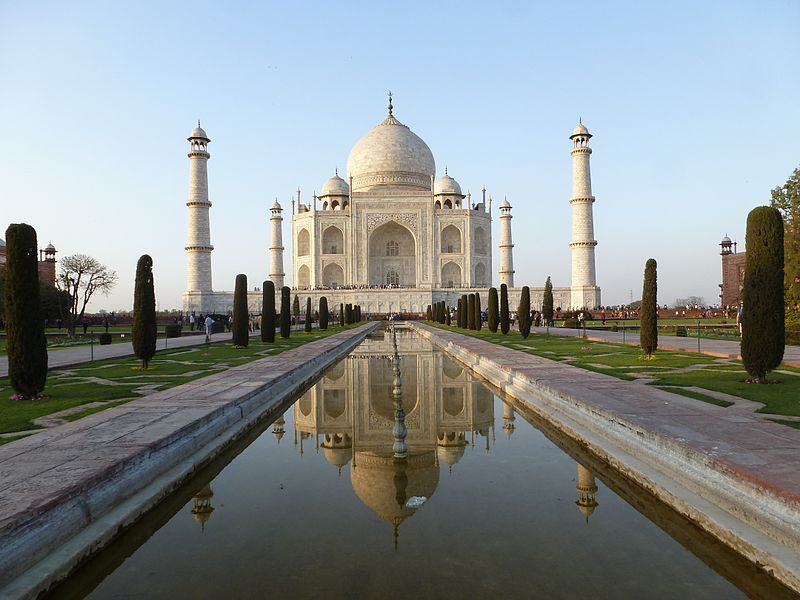
\includegraphics[width=3in]{tajMahal.jpg}
      \end{center}
    \item This picture has $180^\circ$-rotational symmetry,
      as does this picture:
      \begin{center}
        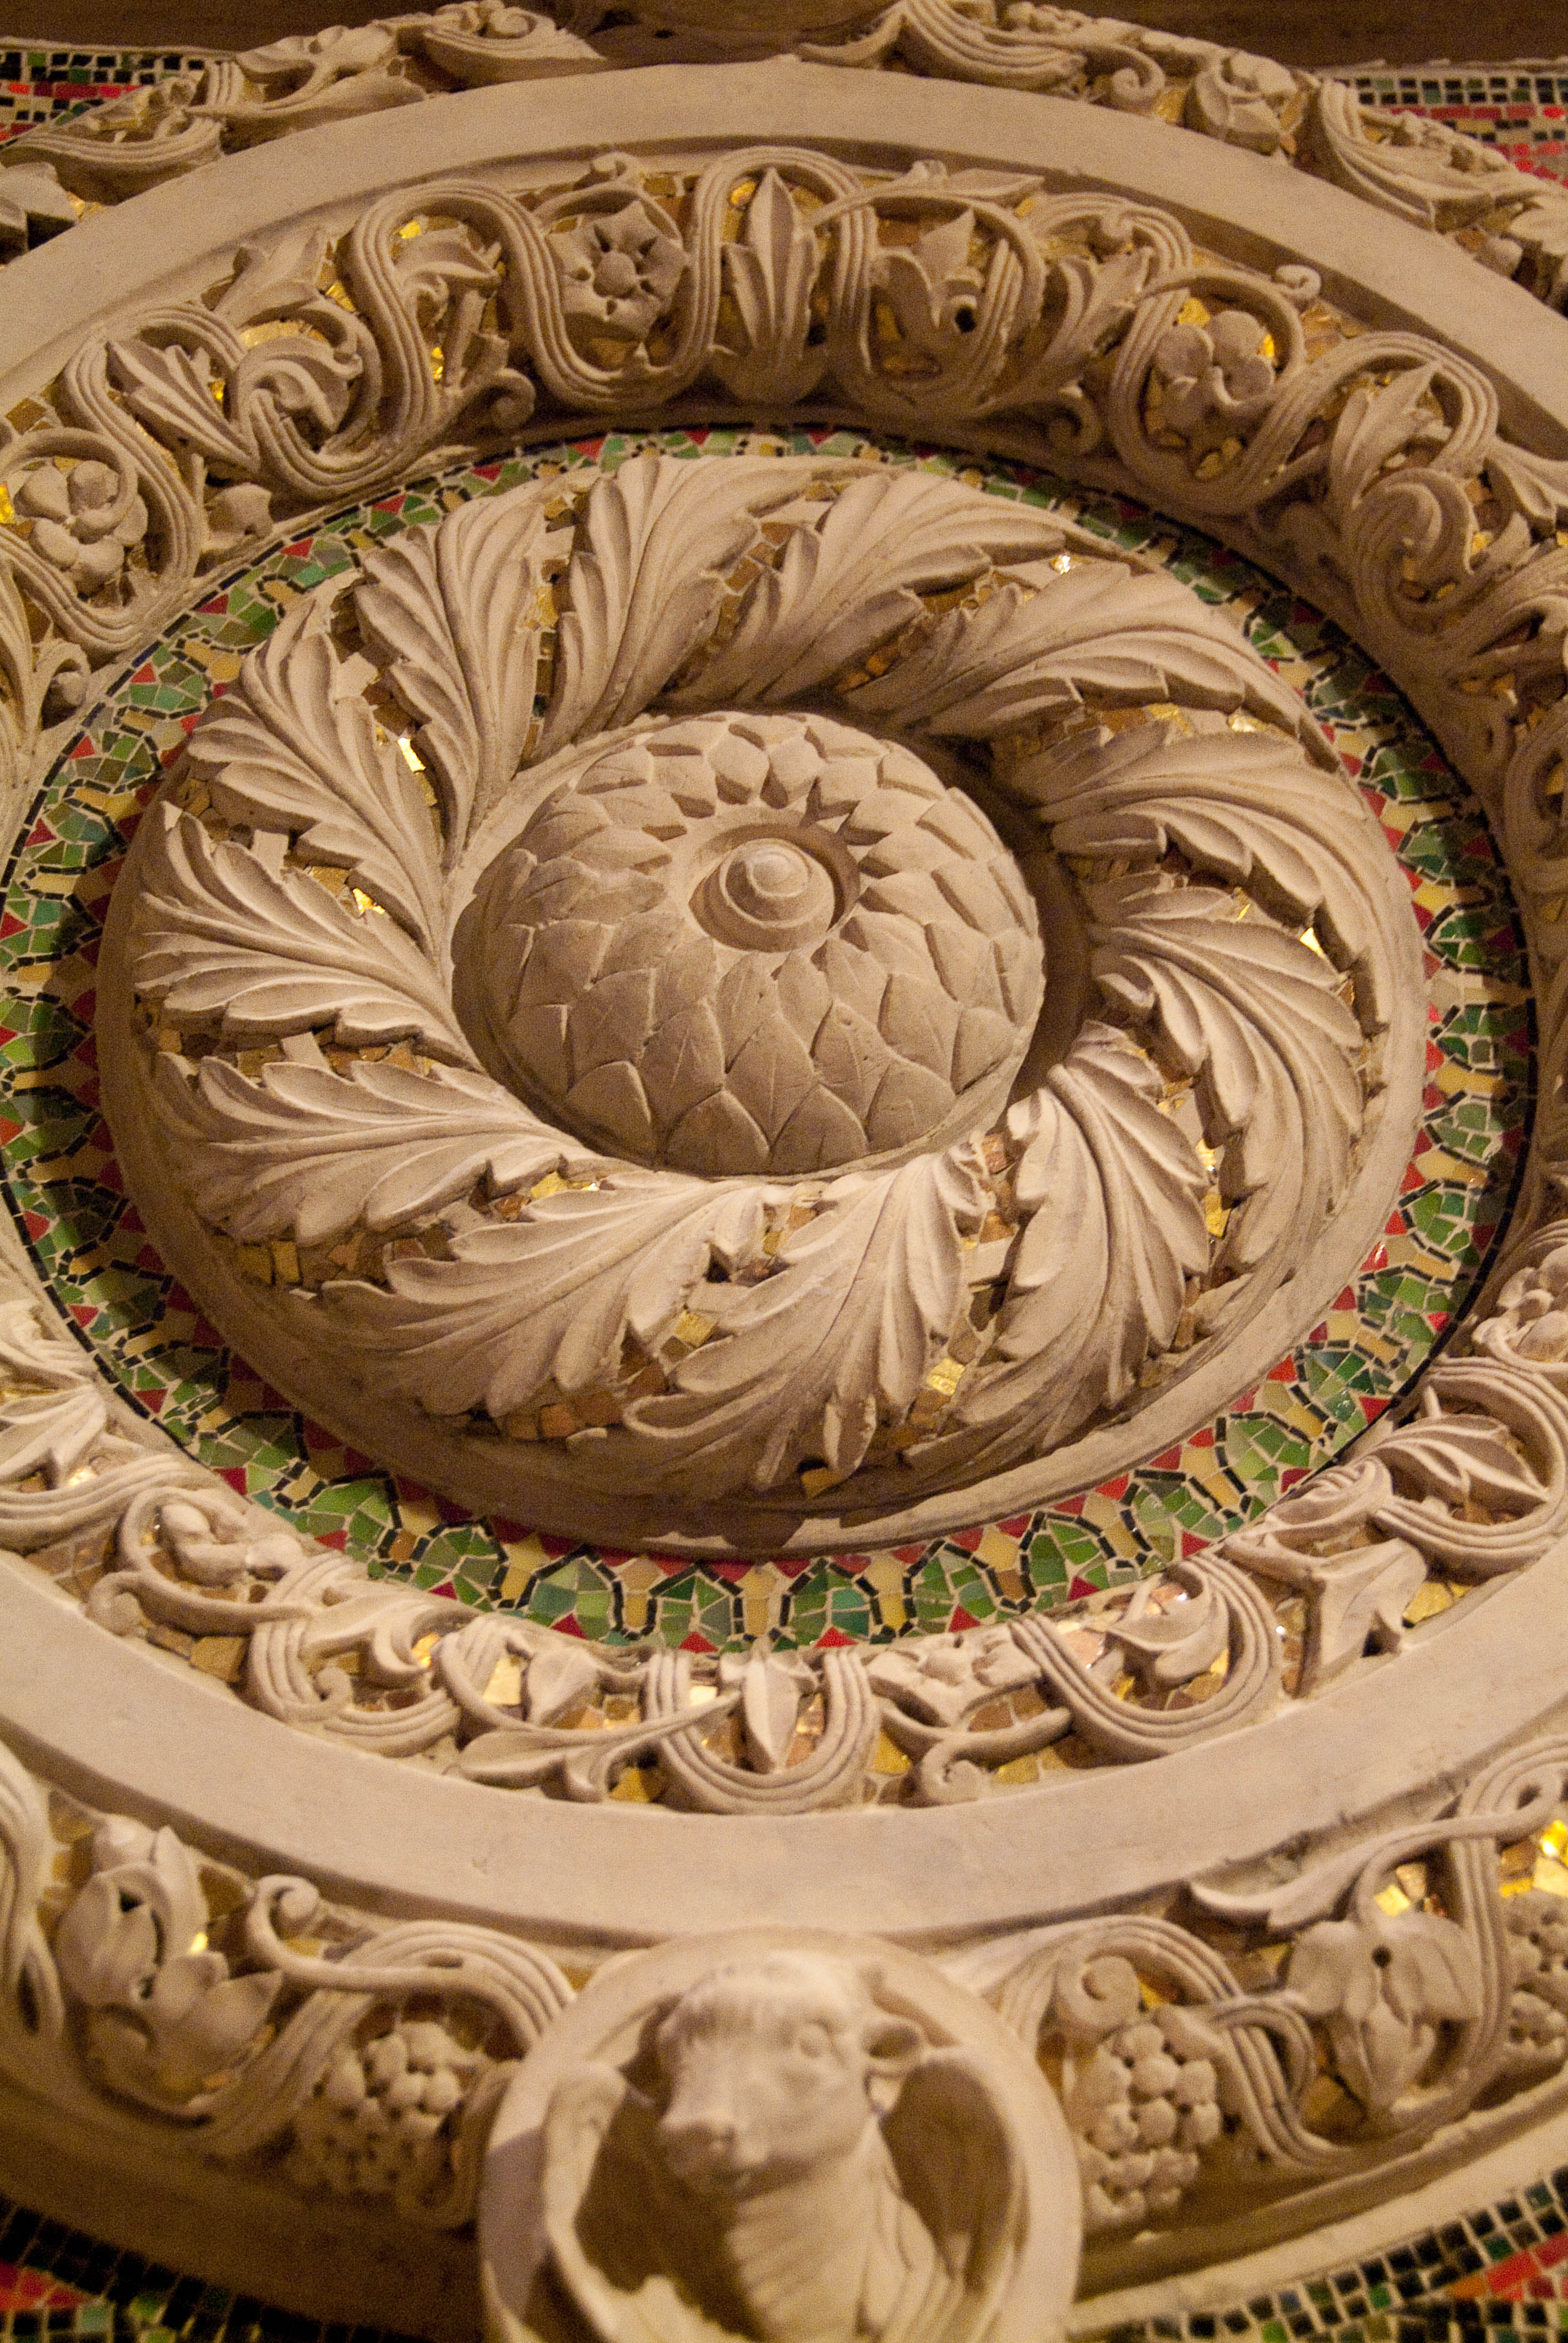
\includegraphics[width=2in]{spin.jpg}
      \end{center}
    \item This picture has symmetry through translations,
      as does this picture:
      \begin{center}
        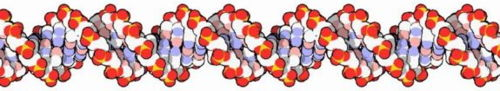
\includegraphics[width=3in]{dna.jpg}
      \end{center}
    \item This picture has symmetry through scaling,
      as does this picture:
      \begin{center}
        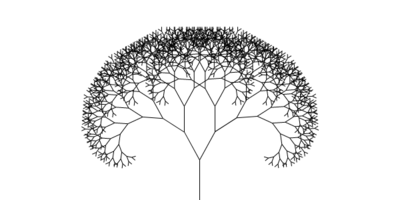
\includegraphics[width=3in]{fractalTree.png}
      \end{center}
    \end{enumerate}
  \end{freeResponse}
\end{question}
\mynewpage


\begin{question}
  Symmetry is ``immunity to change.'' EXPLAIN how this statement is
  TRUE using the EXAMPLES ABOVE. In EACH CASE ABOVE, explain what the
  ``change'' is, and how the example is ``immune'' to the change.
  \begin{freeResponse}
    \begin{enumerate}
      \item The \underline{change} is flipping the picture over a
        vertical line. Since the picture is the same on one side of
        the vertical line, as it is on the other, the picture is
        \underline{immune} to this change.
      \item The \underline{change} is rotating the picture
        $180^\circ$. Since the picture is the same, but backwards, on
        the top as it is on the bottom, the picture is
        \underline{immune} to this change.
      \item The \underline{change} is sliding this picture to the
        right or left. Since the picture is the same, repeated pattern
        is a row, it is \underline{immune} to this change.
      \item The \underline{change} is sliding this picture and scaling
        the picture. Since the picture is the same shape (with the
        same angles), it is \underline{immune} to this change.
    \end{enumerate}
  \end{freeResponse}
\end{question}
\mynewpage



\begin{question}
  For us a \textbf{symmetry} is a function (or ``action,'' or
  ``transformation'') that \textit{somehow} leaves the object it acts
  on unchanged.  In EACH CASE ABOVE what are the functions (or
  ``actions,'' or ``transformations'') of each of these objects that
  leaves them unchanged? USE WORDS TO EXPLAIN HOW THE FUNCTION/ACTION/TRANSFORMATION WORKS.
  \begin{freeResponse}
  \begin{enumerate}
  \item In this case, the function flips the picture over a given
    vertical line
  \item In this case, the function takes a vertical line, and flips the picture over the line.
  \item In this case, the function takes an infinite strip, and slides it to the left or right.
  \item In this case, the function take part of the picture and scales
    it as it slides the picture.
  \end{enumerate}
  \end{freeResponse}
  
\end{question}

\end{document}
